%% ---------------------------------------------------------------------------
%% This file is part of the "Boost Python" talk.
%%
%% Copyright 2015 by Eugen Wintersberger <eugen.wintersberger@gmail.com>
%%
%% This work is licensed under the Creative Commons
%% Attribution-NonCommercial-ShareAlike 4.0 International License. To view 
%% a copy of this license, visit 
%% http://creativecommons.org/licenses/by-nc-sa/4.0/.
%% ---------------------------------------------------------------------------

\section{Creating Python objects}
\begin{frame}{A short overview}
    \begin{itemize}
        \item Python objects: 
            \begin{itemize}
                \item \texttt{object}
                \item \texttt{list}
                \item \texttt{tuple}
                \item \texttt{dictionary}
                \item \texttt{str}
            \end{itemize}
        \item iterator protocols
        \item \texttt{slices}
    \end{itemize}
\end{frame}

\begin{frame}[fragile]{Create native Python objects}
    \texttt{boost::python} provides native implementations for 
    \begin{itemize}
        \item lists \texttt{boost::python::list}
        \item tuples \texttt{boost::python::tuple}
        \item dictionaries \texttt{boost::python::dict}
    \end{itemize}
    \vspace{0.05\textheight}
    \begin{center}
        % Graphic for TeX using PGF
% Title: /home/eugen/Documents/Talks/C++ User Group Hamburg/boost-python/talk2/pics/python_objects.dia
% Creator: Dia v0.97.3
% CreationDate: Mon Apr 18 22:07:50 2016
% For: eugen
% \usepackage{tikz}
% The following commands are not supported in PSTricks at present
% We define them conditionally, so when they are implemented,
% this pgf file will use them.
\ifx\du\undefined
  \newlength{\du}
\fi
\setlength{\du}{15\unitlength}
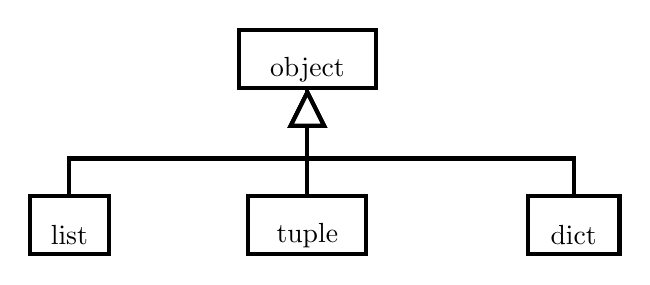
\begin{tikzpicture}
\pgftransformxscale{1.000000}
\pgftransformyscale{-1.000000}
\definecolor{dialinecolor}{rgb}{0.000000, 0.000000, 0.000000}
\pgfsetstrokecolor{dialinecolor}
\definecolor{dialinecolor}{rgb}{1.000000, 1.000000, 1.000000}
\pgfsetfillcolor{dialinecolor}
\pgfsetlinewidth{0.100000\du}
\pgfsetdash{}{0pt}
\definecolor{dialinecolor}{rgb}{1.000000, 1.000000, 1.000000}
\pgfsetfillcolor{dialinecolor}
\fill (24.038750\du,6.000000\du)--(24.038750\du,7.400000\du)--(27.336250\du,7.400000\du)--(27.336250\du,6.000000\du)--cycle;
\definecolor{dialinecolor}{rgb}{0.000000, 0.000000, 0.000000}
\pgfsetstrokecolor{dialinecolor}
\draw (24.038750\du,6.000000\du)--(24.038750\du,7.400000\du)--(27.336250\du,7.400000\du)--(27.336250\du,6.000000\du)--cycle;
% setfont left to latex
\definecolor{dialinecolor}{rgb}{0.000000, 0.000000, 0.000000}
\pgfsetstrokecolor{dialinecolor}
\node at (25.687500\du,6.950000\du){object};
\pgfsetlinewidth{0.100000\du}
\pgfsetdash{}{0pt}
\definecolor{dialinecolor}{rgb}{1.000000, 1.000000, 1.000000}
\pgfsetfillcolor{dialinecolor}
\fill (19.000000\du,10.000000\du)--(19.000000\du,11.400000\du)--(20.907500\du,11.400000\du)--(20.907500\du,10.000000\du)--cycle;
\definecolor{dialinecolor}{rgb}{0.000000, 0.000000, 0.000000}
\pgfsetstrokecolor{dialinecolor}
\draw (19.000000\du,10.000000\du)--(19.000000\du,11.400000\du)--(20.907500\du,11.400000\du)--(20.907500\du,10.000000\du)--cycle;
% setfont left to latex
\definecolor{dialinecolor}{rgb}{0.000000, 0.000000, 0.000000}
\pgfsetstrokecolor{dialinecolor}
\node at (19.953750\du,10.950000\du){list};
\pgfsetlinewidth{0.100000\du}
\pgfsetdash{}{0pt}
\definecolor{dialinecolor}{rgb}{1.000000, 1.000000, 1.000000}
\pgfsetfillcolor{dialinecolor}
\fill (24.266250\du,10.000000\du)--(24.266250\du,11.400000\du)--(27.108750\du,11.400000\du)--(27.108750\du,10.000000\du)--cycle;
\definecolor{dialinecolor}{rgb}{0.000000, 0.000000, 0.000000}
\pgfsetstrokecolor{dialinecolor}
\draw (24.266250\du,10.000000\du)--(24.266250\du,11.400000\du)--(27.108750\du,11.400000\du)--(27.108750\du,10.000000\du)--cycle;
% setfont left to latex
\definecolor{dialinecolor}{rgb}{0.000000, 0.000000, 0.000000}
\pgfsetstrokecolor{dialinecolor}
\node at (25.687500\du,10.950000\du){tuple};
\pgfsetlinewidth{0.100000\du}
\pgfsetdash{}{0pt}
\definecolor{dialinecolor}{rgb}{1.000000, 1.000000, 1.000000}
\pgfsetfillcolor{dialinecolor}
\fill (31.000000\du,10.000000\du)--(31.000000\du,11.400000\du)--(33.205000\du,11.400000\du)--(33.205000\du,10.000000\du)--cycle;
\definecolor{dialinecolor}{rgb}{0.000000, 0.000000, 0.000000}
\pgfsetstrokecolor{dialinecolor}
\draw (31.000000\du,10.000000\du)--(31.000000\du,11.400000\du)--(33.205000\du,11.400000\du)--(33.205000\du,10.000000\du)--cycle;
% setfont left to latex
\definecolor{dialinecolor}{rgb}{0.000000, 0.000000, 0.000000}
\pgfsetstrokecolor{dialinecolor}
\node at (32.102500\du,10.950000\du){dict};
\pgfsetlinewidth{0.100000\du}
\pgfsetdash{}{0pt}
\pgfsetmiterjoin
\pgfsetbuttcap
{
\definecolor{dialinecolor}{rgb}{0.000000, 0.000000, 0.000000}
\pgfsetfillcolor{dialinecolor}
% was here!!!
\definecolor{dialinecolor}{rgb}{0.000000, 0.000000, 0.000000}
\pgfsetstrokecolor{dialinecolor}
\draw (25.687500\du,7.400000\du)--(25.687500\du,9.100000\du)--(19.953750\du,9.100000\du)--(19.953750\du,10.000000\du);
}
\definecolor{dialinecolor}{rgb}{0.000000, 0.000000, 0.000000}
\pgfsetstrokecolor{dialinecolor}
\draw (25.687500\du,8.311803\du)--(25.687500\du,9.100000\du)--(19.953750\du,9.100000\du)--(19.953750\du,10.000000\du);
\pgfsetmiterjoin
\definecolor{dialinecolor}{rgb}{1.000000, 1.000000, 1.000000}
\pgfsetfillcolor{dialinecolor}
\fill (26.087500\du,8.311803\du)--(25.687500\du,7.511803\du)--(25.287500\du,8.311803\du)--cycle;
\pgfsetlinewidth{0.100000\du}
\pgfsetdash{}{0pt}
\pgfsetmiterjoin
\definecolor{dialinecolor}{rgb}{0.000000, 0.000000, 0.000000}
\pgfsetstrokecolor{dialinecolor}
\draw (26.087500\du,8.311803\du)--(25.687500\du,7.511803\du)--(25.287500\du,8.311803\du)--cycle;
% setfont left to latex
\pgfsetlinewidth{0.100000\du}
\pgfsetdash{}{0pt}
\pgfsetmiterjoin
\pgfsetbuttcap
{
\definecolor{dialinecolor}{rgb}{0.000000, 0.000000, 0.000000}
\pgfsetfillcolor{dialinecolor}
% was here!!!
\definecolor{dialinecolor}{rgb}{0.000000, 0.000000, 0.000000}
\pgfsetstrokecolor{dialinecolor}
\draw (25.687500\du,7.400000\du)--(25.687500\du,9.100000\du)--(32.102500\du,9.100000\du)--(32.102500\du,10.000000\du);
}
\definecolor{dialinecolor}{rgb}{0.000000, 0.000000, 0.000000}
\pgfsetstrokecolor{dialinecolor}
\draw (25.687500\du,8.311803\du)--(25.687500\du,9.100000\du)--(32.102500\du,9.100000\du)--(32.102500\du,10.000000\du);
\pgfsetmiterjoin
\definecolor{dialinecolor}{rgb}{1.000000, 1.000000, 1.000000}
\pgfsetfillcolor{dialinecolor}
\fill (26.087500\du,8.311803\du)--(25.687500\du,7.511803\du)--(25.287500\du,8.311803\du)--cycle;
\pgfsetlinewidth{0.100000\du}
\pgfsetdash{}{0pt}
\pgfsetmiterjoin
\definecolor{dialinecolor}{rgb}{0.000000, 0.000000, 0.000000}
\pgfsetstrokecolor{dialinecolor}
\draw (26.087500\du,8.311803\du)--(25.687500\du,7.511803\du)--(25.287500\du,8.311803\du)--cycle;
% setfont left to latex
\pgfsetlinewidth{0.100000\du}
\pgfsetdash{}{0pt}
\pgfsetmiterjoin
\pgfsetbuttcap
{
\definecolor{dialinecolor}{rgb}{0.000000, 0.000000, 0.000000}
\pgfsetfillcolor{dialinecolor}
% was here!!!
\definecolor{dialinecolor}{rgb}{0.000000, 0.000000, 0.000000}
\pgfsetstrokecolor{dialinecolor}
\draw (25.687500\du,7.400000\du)--(25.687500\du,8.250000\du)--(25.687500\du,9.950000\du)--(25.687500\du,10.000000\du);
}
\definecolor{dialinecolor}{rgb}{0.000000, 0.000000, 0.000000}
\pgfsetstrokecolor{dialinecolor}
\draw (25.687500\du,8.311803\du)--(25.687500\du,8.250000\du)--(25.687500\du,9.950000\du)--(25.687500\du,10.000000\du);
\pgfsetmiterjoin
\definecolor{dialinecolor}{rgb}{1.000000, 1.000000, 1.000000}
\pgfsetfillcolor{dialinecolor}
\fill (26.087500\du,8.311803\du)--(25.687500\du,7.511803\du)--(25.287500\du,8.311803\du)--cycle;
\pgfsetlinewidth{0.100000\du}
\pgfsetdash{}{0pt}
\pgfsetmiterjoin
\definecolor{dialinecolor}{rgb}{0.000000, 0.000000, 0.000000}
\pgfsetstrokecolor{dialinecolor}
\draw (26.087500\du,8.311803\du)--(25.687500\du,7.511803\du)--(25.287500\du,8.311803\du)--cycle;
% setfont left to latex
\end{tikzpicture}

    \end{center}
    \vspace{0.05\textheight}
    \texttt{boost::python::object} acts as the base class to all of these.
\end{frame}


\section{Iterators}
\begin{frame}{Iterators}

\end{frame}


\section{Slices}
\begin{frame}{Slice objects}

\end{frame}
